% Contenido integrado por main.tex usando el template suministrado por el usuario.
% Integrar desde docs/report/; requiere graphicx para las dos figuras.
% Informe autocontenido: protocolo, resultados, límites y reproducción.
\section{Problema y alcance}
Construimos un entorno de razonamiento cuantitativo con unidades en español
para preparar el entrenamiento posterior de un modelo pequeño. En este desafío
no se realiza entrenamiento SFT, DPO ni RL. Cada problema se responde en un
turno, sin calculadora, intérprete ni otras herramientas. El prompt proporciona
la fórmula, el valor de $\pi$ cuando corresponde y las equivalencias necesarias;
la tarea exige aplicar operaciones y conversiones, no recordar física.

El objetivo es Qwen3-1.7B. Se comparan Llama 3.2-1B y
SmolLM2-1.7B-Instruct. Qwen3-8B genera las respuestas de entrenamiento y se
evalúa como modelo abierto mayor; no se presenta como modelo de frontera.
DeepSeek-V4-Pro-0813 aporta una referencia externa mediante OpenRouter,
con ruta DeepInfra FP8 y presupuesto de USD 5.

\section{Entorno y generación}
Las familias son velocidad, $v=d/t$; energía cinética, $E=mv^2/2$; y luminosidad,
$L=4\pi d^2F$. Cada familia admite un dato directo o la suma de dos componentes
positivos: distancias, masas o flujos, respectivamente. Esta composición,
las variantes físicas agrupadas y la verificación dimensional constituyen
el aporte acotado del diseño. No se reclama originalidad por cambiar números.
La generación procedural y su verificación tienen antecedentes en Reasoning
Gym, de Stojanovski et al. (2025)~\cite{reasoninggym}; la sensibilidad a variantes
tiene antecedentes en GSM-Symbolic, de Mirzadeh et al. (2024)~\cite{gsmsymbolic}.

El generador final \texttt{units-3} usa distancias de velocidad entre 101 y
9999 m y tiempos entre 7 y 199 s; masas y velocidades entre 1,1 y 49,9 en
kg y m/s. Para luminosidad usa distancias enteras entre 2 y 30 m y flujos
entre 0,01 y 0,99 W/m$^2$. Las componentes de una suma son positivas y su
fracción se encuentra entre 0,2 y 0,8. Los datos visibles se representan con
hasta 15 cifras significativas. Se excluyen cero, valores negativos e
incertidumbres físicas.

Cada problema físico origina tres variantes. Fácil no requiere conversiones;
media requiere una; difícil requiere tres en velocidad y energía, y dos en
luminosidad, cuya salida se solicita en W. Se registran también estructura,
operaciones y representación decimal o científica. Estas etiquetas describen
el diseño; no demuestran una dificultad estrictamente ordenada ni permiten
atribuir causalmente los errores solo a las conversiones.

Se generan 20 grupos por familia con semilla 4301 y se particionan por grupo
con semilla 4302. Cada grupo mantiene juntas sus tres variantes. La identidad
física se define por familia y magnitudes agregadas en SI, incluso cuando
cambia la estructura o la unidad. Se excluyen 95 identidades observadas en
spike, pilotos y controles. Las particiones contienen 90 tareas de train,
36 de eval y 54 de test: respectivamente 10, 4 y 6 grupos por familia.
Cada celda familia/nivel tiene 10, 4 o 6 tareas; las dos estructuras están
balanceadas. Hay 180 tareas, pero solo 60 problemas físicos distintos.

Las referencias son calculadas por código, nunca por el profesor. Un segundo
cálculo interpreta los datos efectivamente impresos en el prompt y comprueba
la referencia con tolerancia relativa $10^{-10}$. Los archivos públicos
omiten las referencias y la clave física; al modelo solo se envía el texto
del prompt. Las plantillas se comparten entre particiones, por lo que el test
evalúa nuevas magnitudes y combinaciones, no generalización a nuevos tipos de
problemas o lenguaje arbitrario.

Por ejemplo, la tarea de train \texttt{14c34d569bd092efd278-medium}
proporciona $d_1=4{,}08$ km, $d_2=1{,}02$ km y $t=88$ s, pide
$v=(d_1+d_2)/t$ y explicita $1$ km$=1000$ m y $1$ m/s$=3{,}6$ km/h.
La referencia privada es $5100/88=57{,}954545\ldots$ m/s. Un resultado
terminal \texttt{57.95 m/s} recibe recompensa; \texttt{0 m/s} no. El prompt
completo pide hasta 80 palabras de explicación en español y un único resultado,
en JSON o cantidad/unidad, sin alternativas. El ejemplo procede de train y
se usa para ilustrar el contrato de respuesta.

\section{Recompensa y robustez}
La interfaz \texttt{reward(prompt, completion) -> float} usa referencias privadas.
Se cargan mediante \texttt{load\_tasks}; un prompt no registrado produce
\texttt{ValueError}. El extractor no recibe la referencia ni ejecuta
expresiones. Admite desarrollo previo y un resultado terminal inequívoco en
JSON con \texttt{value}/\texttt{unit}, o como cantidad y unidad.

El resultado se convierte a SI y recibe recompensa 1 si su dimensión es
compatible, es finito y satisface $|y-y^*|\leq0{,}01|y^*|$; en otro caso,
recibe 0. La tolerancia del 1\% admite redondeo, pero no certifica los pasos.
Se aceptan m/s y km/h; J, kJ y erg; W, kW, erg/s y luminosidades solares,
aunque la unidad difiera de la solicitada. Por tanto, la recompensa no exige
completar la conversión de salida de ciertos niveles difíciles. En test, una
respuesta de Llama aceptada usa km/h donde se pedía m/s; exigir esa unidad
reduciría sus aciertos de cuatro a tres.

Se rechazan alternativas, resultados terminales contradictorios, claves JSON
duplicadas, valores no finitos y unidades incompatibles, sin rescatar números
previos que coincidan con la referencia. Las pruebas usan referencias
independientes: 22 m/s y 79,2 km/h, 9 J y $4\pi$ W. Las etiquetas son
\texttt{correct}, \texttt{numeric}, \texttt{unit} y \texttt{unparsed}; esta última
indica fallo de extracción, no error matemático demostrado. Truncamientos e
intentos incompletos se registran por separado y permanecen en el denominador.

El evaluador \texttt{verifier-9} se congeló antes del test. Incorporó etiquetas
terminales con signo igual y Watts observados en controles de desarrollo:
dos casos pasaron de no interpretados a numéricamente incorrectos, sin nuevos
aciertos ni cambios en piloto o SFT/DPO. Se conservan versiones, hashes e IDs
para distinguir cambios del evaluador de cambios del modelo.

Persisten límites de formato: coma y punto se interpretan como decimales
(\texttt{1,000 J}=1 J; \texttt{3.380 J}=3,38 J), sin convención explícita de
miles en el prompt. Alias como \texttt{joule}, \texttt{kph} y \texttt{Km/h},
números en palabras, ciertos superíndices, LaTeX y expresiones sin evaluar
quedan sin interpretar. La inferencia limita la salida a 1024 tokens, pero
\texttt{reward} no impone un máximo propio de longitud.

Una línea intermedia marcada como resultado y no interpretable puede invalidar
un JSON terminal numéricamente correcto. Se confirmaron tres casos en
Qwen3-1.7B y cuatro en Qwen3-8B. Comprobar solo esos JSON daría 87/162
(53,70\%) y 86/162 (53,09\%), frente a los 84/162 y 82/162 oficiales.
Es un diagnóstico posterior al test, no una validación del razonamiento ni
una corrección de las métricas. Ejemplos: \texttt{a6b709dd46414cbe8a02-hard}
y \texttt{2db7c9328fe1065496fc-hard}, ambos muestra 2.

Se publica cobertura y una cota optimista que trata todas las no interpretadas
como correctas; no es un intervalo de confianza. Antes del entrenamiento se
requieren pruebas adicionales de equivalencias y contradicciones, y políticas
explícitas de unidad, formato numérico, longitud e integración. Una evaluación
independiente de un evaluador ajustado con estos casos requiere un nuevo test
reservado; las recalificaciones sobre las respuestas actuales son análisis
posteriores al test.

\section{Calibración y protocolo experimental}
El piloto inicial, independiente de los datos finales, mostró que luminosidad
quedaba cerca del suelo. Se redujeron sus magnitudes y después se eliminó la
conversión de salida difícil. Se preservaron las respuestas y versiones de
cada piloto; se repitió inferencia cuando cambió el problema y solo se
recalificaron respuestas cuando cambió el evaluador. El piloto consolidado
comprende 90 tareas y 270 respuestas del objetivo: 132 correctas, 126
numéricas incorrectas y 12 no interpretadas; pass@1 de 48,89\%, pass@3 de
65,56\% y cobertura de 95,56\%. Hubo tres truncamientos, uno en
luminosidad difícil; se conservaron en las métricas y respuestas originales.

\begin{figure}[ht]
\centering
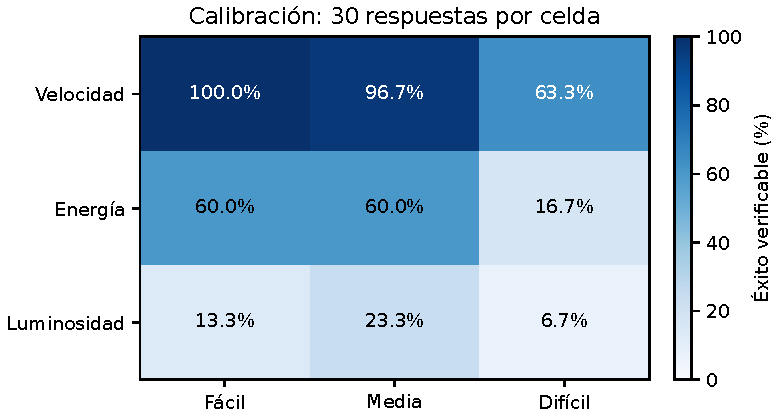
\includegraphics[width=.85\linewidth]{final-v2/figures/calibration.pdf}
\caption{Piloto consolidado del objetivo, previo al congelamiento. Hay 30
respuestas por celda; son variantes relacionadas, no ensayos físicos independientes.}
\end{figure}

Luminosidad difícil permaneció en 2/30 aciertos y se retuvo como estrato de
estrés. Velocidad fácil alcanzó 30/30 y se conservó como control; el nivel
difícil de esa familia tuvo 19/30. Fácil y media no se separaron estrictamente
en el promedio global (57,78\% y 60,00\%).
El núcleo presenta aciertos y errores aprovechables, sin afirmar calibración
suficiente de todas las celdas ni prometer mejora mediante entrenamiento.

El equipo real es Intel Core 5 210H, 12 CPU lógicas, 30,47 GiB de RAM y
NVIDIA RTX 3050 Laptop con 6144 MiB. Driver 595.71.05; NVIDIA-SMI anuncia
compatibilidad máxima CUDA 13.2, que no identifica el runtime usado por
Ollama. El backend es Ollama 0.18.0; Python 3.12.13. Los pesos son GGUF:
Qwen3-1.7B y Qwen3-8B Q4\_K\_M, Llama Q8\_0 y SmolLM2 Q4\_K\_M.
El catálogo conserva digest, licencia, template y metadata efectivamente
observados. Los tamaños del backend (2,0B, 8,2B, 1,2B y 1,7B) difieren de
algunas etiquetas comerciales. Qwen y SmolLM2 declaran Apache-2.0; Llama usa
su Community License~\cite{qwen17,qwen8,llama,smol}.

Se usa un único proceso de inferencia local a la vez. Los parámetros enviados
son temperatura 0,7; top-p 0,9; top-k 40; min-p 0; contexto 2048;
batch 128; solicitud de 99 capas GPU; máximo 1024 tokens; y
\texttt{think=false}. Cada solicitud tiene un mensaje de usuario, sin esquema
JSON forzado. Las semillas son 42, 43 y 44 para la línea base y 42--45 para
train del profesor. Se registran residencia en GPU, duración, tokens y
respuesta completa. Los defaults no controlados se identifican por backend y
template; no se afirma equivalencia de todas las opciones internas.
Los servicios persistentes guardan cada respuesta con sincronización a disco
y reanudan solo claves faltantes con configuración idéntica.

\section{Datos derivados para entrenamiento posterior}
Qwen3-8B produjo cuatro respuestas por cada una de las 90 tareas de train:
360 intentos, 193 aceptados por resultado, 154 errores numéricos y 13 no
interpretados. Tras deduplicar texto por tarea salvo diferencias de espacios,
hubo 178 candidatas correctas distintas. Se seleccionaron cinco candidatas por
familia/nivel con semilla 4303, o todas si había menos. Un defecto obligó a
ampliar la revisión a toda la celda. Además se revisaron todas las candidatas
restantes; finalmente las 178 tienen juicio individual: 121 retenidas y 57
descartadas por calidad contextual. Esta auditoría fue realizada por un
agente auxiliar y contrastada con los artefactos por el agente principal;
no equivale a certificación humana ni a validación por el profesor.

Se conservan 121 trazas SFT de 46 tareas y 20 problemas físicos. Para DPO se emparejan respuestas
retenidas con errores explícitos del mismo prompt, por orden de muestra,
con máximo dos pares por tarea y sin reutilizar chosen ni rejected. No se usa
producto cartesiano. Para completar negativos se consultó al objetivo tres
veces sobre 38 tareas exactas de train: 114 respuestas, 19 errores numéricos
y 6 no interpretadas, que no se usan como negativas. El resultado es 35
pares de 25 tareas y 17 problemas físicos: 22 rechazadas proceden del profesor y 13 del objetivo.

\begin{table}[ht]
\centering
\begin{tabular}{llrr}
Familia & Dificultad & SFT & DPO \\
\midrule
Velocidad & Fácil & 27 & 3 \\
Velocidad & Media & 25 & 4 \\
Velocidad & Difícil & 22 & 11 \\
Energía & Fácil & 13 & 1 \\
Energía & Media & 10 & 5 \\
Energía & Difícil & 1 & 1 \\
Luminosidad & Fácil & 11 & 3 \\
Luminosidad & Media & 11 & 6 \\
Luminosidad & Difícil & 1 & 1 \\
\midrule
Total & & 121 & 35 \\
\end{tabular}
\caption{Datos retenidos por familia y nivel. SFT fácil/media/difícil:
51/46/24; DPO: 7/15/13. Cobertura no equivale a balance suficiente.}
\end{table}

Las cantidades están lejos de las metas orientativas de 4000 SFT y 2000 DPO.
Se priorizó obtener datos trazables y revisar coherencia sin duplicarlos.
La inferencia del profesor tomó 2537,21 s y generó 56563 tokens; media
7,05 s por respuesta. A la retención observada, 4000 SFT proyectarían unas
23,30 horas solo de profesor, sin garantizar igual calidad o diversidad.
Se eligió una escala local acotada antes de congelar los splits. La existencia
de una sola traza en energía y luminosidad difíciles es una limitación material
para el proyecto posterior. No se afirma que estos datos basten para entrenar
con éxito ni que el hardware haga imposible una generación más larga.

\section{Línea base y análisis cualitativo}
El test contiene 54 tareas de 18 problemas físicos, con tres muestras por
modelo. Para una tarea con $c$ aciertos en $n=3$ intentos se usa
$\widehat{\mathrm{pass@}k}=1-\binom{n-c}{k}/\binom{n}{k}$ y se promedia entre
tareas. pass@1 es $c/3$; pass@3 indica al menos un acierto observado. Las
tablas usan porcentajes y se generan de las respuestas guardadas con la misma
versión final del verificador, sin nuevas inferencias. Los tríos no son
observaciones independientes; no se reportan intervalos binomiales que ignoren
esa dependencia.

\begingroup\small\setlength{\tabcolsep}{3pt}
\begin{table}[ht]
\centering
\begin{tabular}{lrrrr}
Modelo & pass@1 [sup.] & pass@3 [sup.] & Cobertura & No interpretadas \\
\midrule
Qwen3-1.7B & 51.85 [56.17] & 68.52 [74.07] & 95.68 & 7 \\
Llama 3.2-1B & 2.47 [58.02] & 7.41 [100.00] & 44.44 & 90 \\
SmolLM2-1.7B & 3.09 [79.63] & 7.41 [100.00] & 23.46 & 124 \\
Qwen3-8B (generador) & 50.62 [54.32] & 72.22 [77.78] & 96.30 & 6 \\
DeepSeek-V4-Pro-0813 & 82.10 [100.00] & 90.74 [100.00] & 82.10 & 29 \\
\end{tabular}
\caption{Línea base: porcentajes sobre 54 tareas y 162 respuestas por modelo. Entre corchetes, cota optimista si todas las no interpretadas fueran correctas; no es intervalo de confianza.}
\label{tab:baseline}
\end{table}
\begin{table}[ht]
\centering
\begin{tabular}{llrr}
Modelo & Dificultad & pass@1 [sup.] & pass@3 [sup.] \\
\midrule
Qwen3-1.7B & Fácil & 62.96 [66.67] & 72.22 [77.78] \\
Qwen3-1.7B & Media & 55.56 [62.96] & 72.22 [83.33] \\
Qwen3-1.7B & Difícil & 37.04 [38.89] & 61.11 [61.11] \\
Llama 3.2-1B & Fácil & 5.56 [57.41] & 16.67 [100.00] \\
Llama 3.2-1B & Media & 0.00 [61.11] & 0.00 [100.00] \\
Llama 3.2-1B & Difícil & 1.85 [55.56] & 5.56 [100.00] \\
SmolLM2-1.7B & Fácil & 1.85 [77.78] & 5.56 [100.00] \\
SmolLM2-1.7B & Media & 5.56 [79.63] & 11.11 [100.00] \\
SmolLM2-1.7B & Difícil & 1.85 [81.48] & 5.56 [100.00] \\
Qwen3-8B (generador) & Fácil & 70.37 [70.37] & 94.44 [94.44] \\
Qwen3-8B (generador) & Media & 62.96 [62.96] & 88.89 [88.89] \\
Qwen3-8B (generador) & Difícil & 18.52 [29.63] & 33.33 [50.00] \\
DeepSeek-V4-Pro-0813 & Fácil & 77.78 [100.00] & 88.89 [100.00] \\
DeepSeek-V4-Pro-0813 & Media & 79.63 [100.00] & 88.89 [100.00] \\
DeepSeek-V4-Pro-0813 & Difícil & 88.89 [100.00] & 94.44 [100.00] \\
\end{tabular}
\caption{Resultados por dificultad: 18 tareas y 54 respuestas por fila. Corchetes: cota optimista de extracción, no intervalo de confianza.}
\label{tab:levels}
\end{table}
\endgroup

\begin{figure}[ht]
\centering
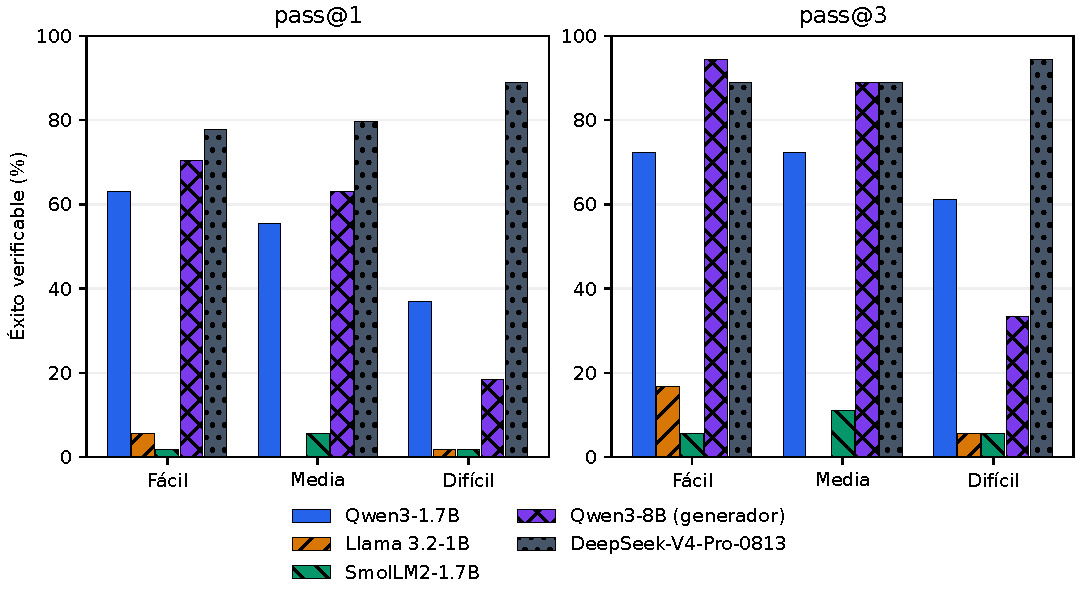
\includegraphics[width=\linewidth]{final-v2/figures/baseline.pdf}
\caption{Evaluación con verificador común por dificultad; 18 tareas y 54 respuestas
por modelo y nivel. Ver cobertura y categorías antes de interpretar diferencias.}
\end{figure}

En el objetivo, pass@1 es 62,96\% en fácil, 55,56\% en media y 37,04\% en
difícil; por familia es 87,04\% en velocidad, 55,56\% en energía y 12,96\%
en luminosidad. La mezcla global no debe ocultar la concentración de dificultad
en la última familia. No hubo truncamientos ni intentos incompletos del backend
en Qwen3-1.7B ni en Llama. SmolLM2 tuvo diez truncamientos y un intento
incompleto, conservados entre sus 162 respuestas; su cobertura fue 23,46\%.
Por ello, su pass@1 automático de 3,09\% es una medida del sistema completo
bajo este contrato, no una estimación fiable de exactitud matemática aislada.
Su cota optimista alcanza 79,63\%, ilustrando la incertidumbre de extracción.
SmolLM2 no tiene aciertos automáticos en energía ni en luminosidad; los cinco
proceden de velocidad. Los ejemplos conservados incluyen el único intento
con \texttt{done=false} y una respuesta que alcanza el límite de 1024 tokens.
Qwen3-8B obtuvo 82 aciertos, 74 errores numéricos y seis no interpretadas:
pass@1 de 50,62\%, pass@3 de 72,22\% y cobertura de 96,30\%, sin truncamientos
ni intentos incompletos. Qwen3-1.7B tuvo 84 aciertos y pass@3 de 68,52\%.
Estas diferencias sobre una muestra pequeña y relacionada no demuestran
superioridad estadística de uno sobre otro. El profesor mayor no garantiza
mejores respuestas ni datos automáticamente coherentes.

Las 648 respuestas locales de test sumaron 2788,28 segundos de solicitudes
y 153259 tokens de salida reportados. Un intento incompleto de SmolLM2 no
informó conteo de tokens; no se le asigna un conteo observado de cero. Por modelo, Qwen3-1.7B consumió 435,12 s y
31521 tokens; Llama, 395,58 s y 26414; SmolLM2, 869,42 s y 71009; y
Qwen3-8B, 1088,16 s y 24315. El costo de API local es cero y no incluye
electricidad. La memoria de modelo reportada por Ollama residió completamente
en GPU en las 162 observaciones de cada modelo; no se atribuye esa cifra
al tamaño de los pesos en disco ni a toda la memoria del proceso.

En Qwen3-1.7B, una respuesta suma 2,936 y 0,734 km, convierte a 3670 m y
divide por 150 s para obtener 24,47 m/s correctamente. Otra trata 0,25 min
como 0,25 s y produce un resultado 60 veces mayor. En energía, 1022,27 J
recibe aceptación frente a 1016,452 J por quedar dentro del 1\%, aunque
la multiplicación descrita es incorrecta. En luminosidad, una respuesta
termina correctamente en 30,7876 W pero afirma falsamente que
1 W equivale a 1000 erg/s: el número final no certifica razonamiento dimensional.
Un párrafo con cálculo y redondeo coherentes termina en una estructura
LaTeX no admitida y permanece \texttt{unparsed}; no se modifica su etiqueta.

Los ejemplos cualitativos conservan ID, índice de muestra, hash y juicio
automático. Son ilustraciones seleccionadas, no una estimación de frecuencia
de causas ni una corrección manual de las métricas. La baja cobertura de
Llama, particularmente en luminosidad, impide atribuir todos sus fallos
automáticos a capacidad matemática. Cuantizaciones y templates distintos,
el idioma español y la configuración de pensamiento limitan la atribución
causal de las diferencias a parámetros o familias de modelos.

\subsection{Referencia externa}
DeepSeek-V4-Pro-0813~\cite{deepseek} se evaluó mediante OpenRouter con ruta
DeepInfra FP8 fija, sin fallback, bajo un presupuesto de USD 5. El catálogo
conserva precios y parámetros; el proveedor nativo quedó excluido por la
política de privacidad de la cuenta. Cinco controles ajenos a test produjeron
tres aciertos y dos no interpretadas, sin truncamientos, por USD 0,0029965;
no se ajustó el parser a sus resultados.

Se usaron los mismos 54 prompts, tres muestras, máximo 1024 tokens,
temperatura 0,7, top-p 0,9, top-k 40, min-p 0 y semillas 42--44; razonamiento
desactivado, sin herramientas ni JSON forzado. El contexto anunciado es
1048576 tokens, frente a 2048 locales. El modelo fechado y proveedor identifican
la revisión remota, sin digest de pesos observable; FP8 procede del catálogo.
Estos motores y sus defaults impiden asumir equivalencia de muestreo o
reproducibilidad bit a bit.

El test produjo 133 aciertos y 29 no interpretadas: pass@1 de 82,10\%,
pass@3 de 90,74\% y cobertura de 82,10\%. No hubo errores numéricos ni de
unidad clasificados, truncamientos o intentos incompletos. Las no interpretadas
impiden concluir exactitud matemática perfecta y elevan ambas cotas optimistas
a 100\%. Fácil/media/difícil alcanzaron 77,78/79,63/88,89\% en pass@1;
los niveles no ordenan universalmente la capacidad. Entre los falsos negativos,
una respuesta obtiene 410,6 km/h correctamente, pero mencionar que pi no se usa
activa la guardia de negación; otra presenta JSON correcto tras un marcador
narrativo sin cantidad. Se conservan sus etiquetas automáticas.

Las 162 solicitudes consumieron 25377 tokens de entrada y 22125 de salida,
sin tokens de razonamiento reportados: 341,14 s y USD 0,0905151; con controles,
USD 0,0935116. La tarifa capturada fue USD 1,30/2,60 por millón de tokens
entrada/salida~\cite{routing,pricing}. Un registro global reserva USD 0,02 por
intento, incluso fallido, con caps de tarifa 1,32/3,96, prompts de hasta 2048
bytes y margen de 6144 tokens de entrada/1024 de salida. Los 168 intentos,
incluido un rechazo previo a generar, reservaron USD 3,36; reserva y facturación
son magnitudes distintas. La ruta del registro queda vinculada a la
configuración para impedir reinicios accidentales del contador. Su corrección,
probada por regresión simulada, no cambió etiquetas, métricas ni verificador.

\section{Reproducción}
El paquete autocontenido incluye código, pruebas, tareas, SFT/DPO, respuestas,
metadatos e informe. El núcleo usa biblioteca estándar; Matplotlib 3.11.2 y sus
dependencias están fijados para generar figuras. Los manifiestos SHA-256
identifican datos, configuración y código; se preservan versiones y recálculos.
Las pruebas cubren referencias independientes, equivalencias, ataques,
separación de grupos, reanudación y procedencia SFT/DPO.

La guía incluida permite comprobar hashes, regenerar particiones, reconstruir
SFT/DPO y recalcular etiquetas, métricas y PDF desde una copia aislada, sin
pesos ni credenciales. Repetir inferencia requiere los modelos y backends
identificados; igual semilla no garantiza idénticas respuestas entre versiones
o hardware. El costo local excluye electricidad. No se realizó entrenamiento.

\begingroup\raggedright
\begin{thebibliography}{9}
\bibitem{reasoninggym} Z. Stojanovski, O. Stanley, J. Sharratt, R. Jones,
A. Adefioye, J. Kaddour y A. K\"opf. Reasoning Gym: Reasoning Environments
for Reinforcement Learning with Verifiable Rewards. arXiv:2505.24760, 2025.
\url{https://arxiv.org/abs/2505.24760}.
\bibitem{gsmsymbolic} I. Mirzadeh, K. Alizadeh, H. Shahrokhi, O. Tuzel,
S. Bengio y M. Farajtabar. GSM-Symbolic: Understanding the Limitations
of Mathematical Reasoning in Large Language Models. arXiv:2410.05229, 2024.
\url{https://arxiv.org/abs/2410.05229}.
\bibitem{qwen17} Qwen. Qwen3-1.7B, model card oficial. Hugging Face,
\texttt{Qwen/Qwen3-1.7B}. Consulta: 7 de noviembre de 2026.
\bibitem{qwen8} Qwen. Qwen3-8B, model card oficial. Hugging Face,
\texttt{Qwen/Qwen3-8B}. Consulta: 7 de noviembre de 2026.
\bibitem{llama} Meta. Llama-3.2-1B-Instruct, model card oficial. Hugging Face,
\texttt{meta-llama/Llama-3.2-1B-Instruct}. Consulta: 7 de noviembre de 2026.
\bibitem{smol} Hugging Face. SmolLM2-1.7B-Instruct, model card oficial.
\texttt{HuggingFaceTB/SmolLM2-1.7B-Instruct}. Consulta: 7 de noviembre de 2026.
\bibitem{deepseek} DeepSeek / OpenRouter. DeepSeek V4 Pro 0813.
\url{https://openrouter.ai/deepseek/deepseek-v4-pro-20260813}.
Consulta: 7 de noviembre de 2026.
\bibitem{routing} OpenRouter. Provider Routing.
\url{https://openrouter.ai/docs/guides/routing/provider-selection}.
Consulta: 7 de noviembre de 2026.
\bibitem{pricing} OpenRouter. Pricing.
\url{https://openrouter.ai/pricing}. Consulta: 7 de noviembre de 2026.
\end{thebibliography}
\endgroup
